% ============================= MATERIAIS E METODOS ============================
\section{Materiais e métodos}\label{sec:metodos}

\subsection{Desenho do estudo e definição da tarefa}
O estudo é uma comparação retrospectiva de modelos de predição clínica, relatada segundo o TRIPOD+AI \cite{collins2024tripodai}. A unidade de análise é o paciente, com uma linha por pessoa e todas as variáveis medidas na data de registro no estudo (linha de base). A tarefa é a classificação binária de óbito em até cinco anos (1.826 dias). O rótulo foi definido assim: pacientes que morreram até 1.826 dias recebem 1; pacientes acompanhados por mais de 1.826 dias, vivos ou mortos depois disso, recebem 0; pacientes censurados ou transplantados antes de 1.826 dias são excluídos, porque não se sabe se teriam morrido no horizonte. Classificar com horizonte fixo, em vez de modelar o tempo até o evento, permite comparar diretamente modelos de classificação e o escore de Cox na mesma métrica, ao custo de excluir esses pacientes.

O desenho é 2 x 2: duas famílias de métodos (regressão e AM), cada uma com as 5 variáveis do Escore de Mayo e com as 17 variáveis do conjunto, nos mesmos pacientes e nas mesmas partições. A leitura horizontal (mesma família) mostra o efeito das variáveis extras. A leitura vertical (mesmas variáveis) compara pipelines, que diferem no algoritmo e também no tratamento dos dados; uma análise de sensibilidade aproxima a comparação do efeito do algoritmo ao dar às árvores o pré-processamento da regressão.

\subsection{Conjunto de dados e caracterização da amostra}\label{subsec:dados}
O conjunto é o \textit{Cirrhosis Patient Survival Prediction} do repositório da UCI (identificador 878, licença CC BY 4.0) \cite{uci878}, que reproduz os dados do ensaio da Mayo Clinic sobre D-penicilamina em CBP, realizado entre 1974 e 1984 e acompanhado até julho de 1986 \cite{dickson1989prognosis,fleming1991counting}. São 418 pacientes: 312 participaram do ensaio randomizado, e 106 eram elegíveis, recusaram a randomização e só têm as medidas de rotina. São 374 mulheres (89,5\%). O desfecho original tem três classes: censura (232), óbito (161) e transplante (25), com o tempo até o desfecho em dias (\texttt{N\_Days}). A Tabela~\ref{tab:variaveis} descreve as variáveis.

\begin{table}[htbp]
\centering
\caption{Variáveis do conjunto de dados e seu uso no estudo.}
\label{tab:variaveis}
\small
\renewcommand{\arraystretch}{1.12}
\begin{tabularx}{\linewidth}{@{}p{3.6cm}p{2.0cm}p{2.3cm}X@{}}
\toprule
\textbf{Variável} & \textbf{Tipo} & \textbf{Função} & \textbf{Definição e codificação} \\
\midrule
Idade, bilirrubina, albumina, tempo de protrombina, edema & Numéricas e ordinal & Preditores (5 de Mayo) & Idade em anos; exames em mg/dL, g/dL e segundos; edema em 0, 0,5 e 1, como no escore \\
Colesterol, cobre urinário, fosfatase alcalina, AST, triglicerídeos, plaquetas & Numéricas & Preditores (17 var.) & Exames laboratoriais da linha de base \\
Sexo, ascite, hepatomegalia, aranhas vasculares & Binárias & Preditores (17 var.) & Sinais clínicos em 0 ou 1 \\
Tratamento, estágio histológico & Binária e ordinal & Preditores (17 var.) & D-penicilamina ou placebo; estágio de 1 a 4 \\
\texttt{Status} & Categórica & Construção do alvo & Censura, óbito ou transplante \\
\texttt{N\_Days} & Numérica & Construção do alvo; possível vazamento & Dias até o desfecho; nunca usada como entrada, exceto no braço de controle \\
\bottomrule
\end{tabularx}
\par\vspace{3pt}{\footnotesize\color{cinzasec}Fonte: elaboração própria a partir de \citeonline{uci878}.}
\end{table}

\subsection{Pipeline de preparação e modelagem}\label{subsec:pipeline}
A Figura~\ref{fig:pipeline} resume o fluxo. Todas as transformações que dependem dos dados (imputação, padronização e ajuste de hiperparâmetros) ficam dentro de um \textit{pipeline} do \textit{scikit-learn} \cite{pedregosa2011scikit} e são reaprendidas no treino de cada partição. Na regressão logística, os exames de distribuição assimétrica entram em logaritmo natural, como no Escore de Mayo, seguidos de padronização. As 5 variáveis de Mayo têm apenas 2 pacientes rotulados com algum valor ausente, imputados pela mediana do treino. Para as 17 variáveis, usou-se imputação iterativa por equações encadeadas \cite{vanbuuren2011mice}, na escala logarítmica para a regressão e na escala original para o \textit{random forest}. O XGBoost trata ausentes nativamente. Não houve balanceamento artificial de classes, que distorceria as probabilidades previstas \cite{christodoulou2019systematic}.

\begin{figure}[htbp]
\centering
\begin{tikzpicture}[
  >=Latex,
  etapa/.style={draw=azulescuro!36,rounded corners=2.5pt,fill=azulclaro,
    align=center,text width=2.97cm,minimum height=1.08cm,font=\footnotesize\sffamily},
  seta/.style={->,line width=.7pt,draw=azulescuro!65}
]
\node[etapa] (a) {UCI 878: 418\\pacientes, 17 variáveis};
\node[etapa,right=0.25cm of a] (b) {Rótulo de 5 anos:\\312 pacientes, 115 óbitos};
\node[etapa,right=0.25cm of b] (c) {Validação cruzada\\5 x 5, mesmas partições};
\node[etapa,below=0.65cm of c] (d) {Imputação e escala\\aprendidas no treino};
\node[etapa,left=0.25cm of d] (e) {Busca aninhada:\\12 configurações};
\node[etapa,left=0.25cm of e] (f) {AUROC, calibração e\\valor incremental};
\draw[seta] (a)--(b); \draw[seta] (b)--(c); \draw[seta] (c)--(d);
\draw[seta] (d)--(e); \draw[seta] (e)--(f);
\end{tikzpicture}
\caption{Pipeline do experimento principal.}
\label{fig:pipeline}
\par\vspace{3pt}{\footnotesize\color{cinzasec}Fonte: elaboração própria.}
\end{figure}

\subsection{Análise exploratória dos dados}
Dos 418 pacientes, 312 receberam rótulo (115 óbitos em até cinco anos, 36,9\%) e 106 foram excluídos (89 censurados e 17 transplantados antes do horizonte). Coincidentemente, os excluídos também são 106, mas não são os 106 pacientes fora do ensaio: dos 312 rotulados, 68 não participaram da randomização. A prevalência de óbito de 36,9\% não exige métricas para eventos raros, mas torna a calibração tão importante quanto a discriminação. A ausência de dados se concentra nas variáveis colhidas só no ensaio: tratamento, ascite, hepatomegalia, aranhas, fosfatase alcalina e AST faltam para os 106 pacientes não randomizados, e colesterol e triglicerídeos faltam também em cerca de 30 pacientes do ensaio. Por isso, dos 312 rotulados, 310 têm as 5 variáveis de Mayo completas e só 210 têm as 17. A Figura~\ref{fig:ndays} mostra por que \texttt{N\_Days} vaza informação: a mediana do tempo é bem menor nos óbitos do que nos censurados, de modo que o tempo de seguimento carrega o próprio desfecho.

\begin{figure}[htbp]
\centering
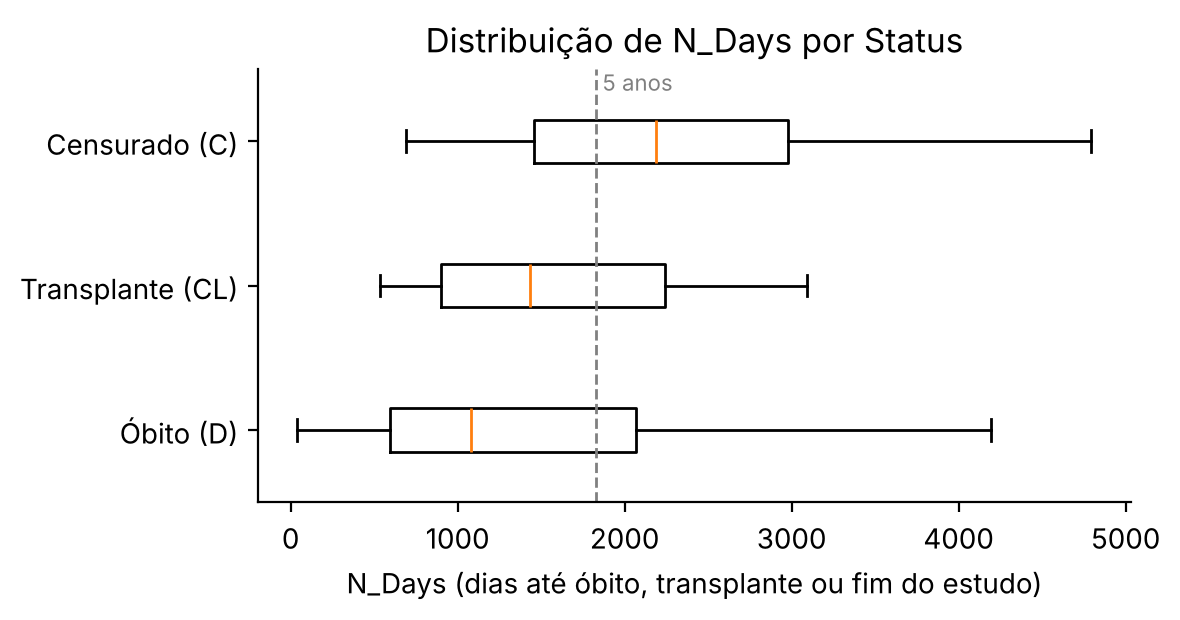
\includegraphics[width=0.72\linewidth]{figuras/n_days_por_status.png}
\caption{Distribuição do tempo de seguimento (\texttt{N\_Days}) por desfecho; a linha tracejada marca o horizonte de cinco anos.}
\label{fig:ndays}
\par\vspace{3pt}{\footnotesize\color{cinzasec}Fonte: elaboração própria a partir de \citeonline{uci878}; 418 pacientes.}
\end{figure}

\subsection{Estratégia de validação e prevenção de vazamento}
A avaliação principal usa validação cruzada estratificada repetida, com 5 repetições de 5 partições (25 avaliações) e as mesmas divisões para todos os modelos. O ajuste de hiperparâmetros é aninhado \cite{varma2006bias}: em cada partição externa, uma busca aleatória com 3 partições internas, critério AUROC e 12 configurações sorteadas usa só o treino. A predição fora da partição de cada paciente é a média das 5 repetições. A variável \texttt{N\_Days} nunca é entrada, porque só é conhecida depois do desfecho.

Duas análises complementares testam a generalização e o vazamento. Na validação quase externa, os modelos são desenvolvidos nos 244 pacientes rotulados do ensaio randomizado (85 óbitos, 34,8\%) e testados nos 68 rotulados não randomizados (30 óbitos, 44,1\%). Nesse teste, as variáveis exclusivas do ensaio estão ausentes e são imputadas ou tratadas nativamente. No braço de controle de vazamento, o enquadramento da competição do Kaggle é reproduzido: classificação de \texttt{Status} em três classes nos 418 pacientes, com XGBoost e as 17 variáveis, com e sem \texttt{N\_Days} como entrada, na mesma validação 5 x 5.

\subsection{Algoritmos e ajuste de hiperparâmetros}
Seja $\mathbf{x}_i$ o vetor de variáveis de linha de base do paciente $i$ e $y_i \in \{0,1\}$ o indicador de óbito em até cinco anos. Cada modelo estima $\hat{\pi}(\mathbf{x}) = \hat{P}(y=1 \mid \mathbf{x})$.

\textbf{Escore de Mayo (referência histórica).} O modelo final de \citeonline{dickson1989prognosis}, estimado com os 418 pacientes, define o escore
\begin{equation}
\begin{aligned}
R ={}& 0{,}039\,\text{idade} + 0{,}871\ln(\text{bilirrubina}) - 2{,}53\ln(\text{albumina})\\
&+ 2{,}38\ln(\text{protrombina}) + 0{,}859\,\text{edema},
\end{aligned}
\label{eq:mayo}
\end{equation}
e a implementação reproduz os dois exemplos resolvidos do artigo original ($R = 3{,}12$ e $R = 8{,}39$). A probabilidade original de óbito em cinco anos é $\hat{\pi} = 1 - 0{,}774^{\exp(R - 5{,}07)}$, em que 0,774 é a sobrevida basal em cinco anos e 5,07 é a média de $R$ na coorte. Como esses coeficientes foram estimados nos mesmos pacientes usados aqui, inclusive nos de teste, o escore publicado entra apenas como referência histórica, em duas versões: a probabilidade original e uma versão recalibrada no treino, $\hat{\pi} = \sigma(a + bR)$, com $\sigma(z) = 1/(1+e^{-z})$. Na validação quase externa entra também o modelo inicial de \citeonline{dickson1989prognosis}, estimado só com os 312 pacientes randomizados e, portanto, sem contato com o teste.

\textbf{Regressão logística com as 5 variáveis de Mayo (referência principal).} O modelo $\hat{\pi}(\mathbf{x}) = \sigma(\beta_0 + \boldsymbol{\beta}^\top \tilde{\mathbf{x}})$, com as variáveis transformadas e padronizadas $\tilde{\mathbf{x}}$, é estimado por máxima verossimilhança em cada partição. É o Escore de Mayo reestimado, livre do vazamento dos coeficientes publicados.

\textbf{Regressão logística com 17 variáveis.} Penalização \textit{elastic net} \cite{zou2005elasticnet}, que minimiza a perda logística mais $\frac{1}{C}\big(\alpha\|\boldsymbol{\beta}\|_1 + \frac{1-\alpha}{2}\|\boldsymbol{\beta}\|_2^2\big)$, com $C \in \{0{,}01;\,0{,}03;\,0{,}1;\,0{,}3;\,1;\,3\}$ e $\alpha \in \{0;\,0{,}5;\,1\}$.

\textbf{\textit{Random forest}.} Média de 300 árvores de classificação, cada uma treinada numa amostra \textit{bootstrap} e escolhendo cada divisão entre um subconjunto aleatório de variáveis \cite{breiman2001random}. Grade: tamanho mínimo da folha em $\{3, 5, 10, 20\}$, variáveis por divisão em $\{\sqrt{p}, 0{,}5p, p\}$ e profundidade em $\{$livre$, 4, 6\}$.

\textbf{XGBoost.} Modelo aditivo de árvores ajustadas por gradiente com aproximação de segunda ordem e regularização \cite{chen2016xgboost}. Grade: número de árvores em $\{100, 200, 400\}$, taxa de aprendizado em $\{0{,}02;\,0{,}05;\,0{,}1\}$, profundidade em $\{1, 2, 3\}$, peso mínimo por folha em $\{1, 5\}$ e regularização L2 em $\{1, 5\}$.

Nas tabelas, RL designa a regressão logística e RF, o \textit{random forest}. As grades foram definidas antes de qualquer resultado e não foram alteradas depois. Todos os modelos com busca usam o mesmo orçamento de 12 configurações. Na análise de sensibilidade, \textit{random forest} e XGBoost com 17 variáveis recebem exatamente o pré-processamento da regressão com 17 variáveis (logaritmo, imputação iterativa e padronização). Como árvores são invariantes a transformações monotônicas, a diferença restante em relação à regressão é o algoritmo com seus hiperparâmetros.

\subsection{Métricas de avaliação}\label{subsec:metricas}
A métrica principal é a área sob a curva ROC (AUROC), a probabilidade de o modelo atribuir risco maior a um paciente que morreu do que a um que sobreviveu \cite{fawcett2006roc}. Complementam a discriminação a precisão média (AP, soma da precisão ponderada pelos incrementos de revocação) e, num limiar de 0,5, precisão, sensibilidade (revocação), especificidade e F1. A sensibilidade é
\begin{equation}
\operatorname{Sensibilidade}=\frac{VP}{VP+FN},
\label{eq:sensibilidade}
\end{equation}
em que $VP$ é o número de verdadeiros positivos e $FN$ o de falsos negativos. A exatidão das probabilidades é medida pelo escore de Brier, $\frac{1}{n}\sum_i(\hat{\pi}_i - y_i)^2$, e pela calibração \cite{vancalster2019calibration}. A calibração no geral (CITL) é o intercepto $a$ em $\operatorname{logit} P(y=1) = a + \operatorname{logit}(\hat{\pi})$, ajustado com o logito da predição como \textit{offset}; o ideal é 0, valores positivos indicam subestimação do risco e negativos, superestimação. A inclinação de calibração é o coeficiente $b$ em $\operatorname{logit} P(y=1) = a + b\,\operatorname{logit}(\hat{\pi})$; o ideal é 1, e valores acima de 1 indicam probabilidades comprimidas demais.

O valor incremental é a diferença de AUROC ($\Delta$AUROC) entre cada modelo e a referência, calculada sobre as predições fora da partição. Os intervalos de confiança vêm de 2.000 reamostragens \textit{bootstrap} pareadas de pacientes. Para as cinco comparações principais, além do IC 95\%, calcula-se um IC simultâneo de Bonferroni de 99\% (nível $1 - 0{,}05/5$), e só se afirma ``maior'' ou ``menor'' quando ele exclui zero. Esses intervalos são condicionais às predições já obtidas, isto é, não incorporam a variação de refazer o treino e a busca de hiperparâmetros, e por isso são exploratórios. Como nenhuma margem de equivalência foi definida a priori, ``sem evidência de diferença'' não significa equivalência. A variação do treino aparece na dispersão da diferença de AUROC entre as 25 partições.

\subsection{Reprodutibilidade e aspectos éticos}
O experimento foi executado em Python 3.13 com scikit-learn 1.9.1 e XGBoost 3.4.1, com versões fixadas, semente 2026 em todos os componentes aleatórios e verificação SHA-256 da cópia dos dados. Os hiperparâmetros escolhidos em cada partição foram salvos, e nenhum aviso de convergência ocorreu. Duas execuções completas do notebook, guardadas em commits distintos do repositório, produziram os mesmos resultados, com diferença absoluta máxima de $1{,}6 \times 10^{-13}$; o script de comparação e sua saída estão em \texttt{auditoria/}. Código, notebook, dados e resultados estão em \url{https://github.com/claytonchagas/ml4health}, e o código e as conclusões passaram por duas rodadas de auditoria independente por outro agente de IA. Os dados são públicos, anonimizados e licenciados para reúso, o que dispensa aprovação ética para esta análise secundária.
